\section{Probabilistic Programming is Everywhere}

% =====================================================================
%  Slide group 1: motivation -- probabilistic programming is everywhere
% =====================================================================

% --- Frame 1.0: applications in the wild ------------------------------
\begin{frame}{Probabilistic programming is everywhere}
  \emph{The most general feature of a PPL --- sampling from a distribution ---
  lives in the standard library of every major language.}
  \medskip

  \begin{columns}[T]
    \begin{column}{0.5\textwidth}
      \begin{itemize}
        \item \wprob{Cryptography} --- protocols, ZK proofs
        \item \wprob{Differential privacy}
        \item \wprob{Randomised algorithms}
        \item \wprob{Distributed systems}
      \end{itemize}
    \end{column}
    \begin{column}{0.5\textwidth}
      \begin{itemize}
        \item \wprob{Bayesian inference} \& probabilistic ML
        \item \wprob{Scientific simulation} --- climate, physics
        \item \wprob{Robotics \& perception} --- intuitive physics
      \end{itemize}
    \end{column}
  \end{columns}

  \vfill
  \begin{center}
    % ---------------------------------------------------------------
    %  PLACEHOLDER FIGURE -- swap this single line for the final image.
    %  (intuitive physics engine: predict whether a block tower falls)
    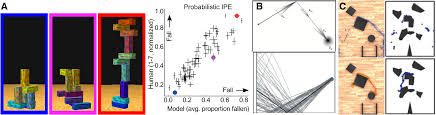
\includegraphics[width=0.62\textwidth]{figs/placeholders/ipe_physics.png}
    % ---------------------------------------------------------------
    \\[-0.2em]
    {\tiny\itshape Placeholder: intuitive physics engine --- probabilistic
     perception predicts ``will it fall?''}
  \end{center}
\end{frame}

% --- Frame 1.1: discrete vs continuous, framed by applications --------
\begin{frame}{Discrete vs.\ continuous}
  The dividing line that matters runs through the \alert{applications}.
  \medskip

  \begin{columns}[T]
    \begin{column}{0.48\textwidth}
      \begin{block}{Discrete}
        Coin flips, Bernoulli / categorical choices, dice.
        \medskip

        Cryptography, differential privacy, randomised algorithms ---
        Applications traditionally within CS - much larger focus.
      \end{block}
    \end{column}
    \begin{column}{0.48\textwidth}
      \begin{block}{Continuous}
        Gaussian noise, sensor models, Bayesian priors over $\mathbb{R}$,
        physical quantities.
        \medskip

        Scientific simulation, Bayesian inference, ML --- where the
        \alert{real-world modelling} happens.
      \end{block}
    \end{column}
  \end{columns}

  \vfill
  \begin{center}
    Continuous distributions are where prior verification work fell short ---\\
    and where this project makes its \wfound{first mechanised} contribution.
  \end{center}
\end{frame}

% --- Frame 1.2: verification is notoriously hard ----------------------
\begin{frame}{Verifying probabilistic programs is notoriously hard}
  \begin{itemize}
    \item Conventional \alert{testing fails}: a rare \emph{correct} outlier
          execution and a genuine bug look \emph{identical}.
    \item Correctness is a property of the whole \alert{distribution}, not of
          any single run.
    \item Reasoning about \alert{independence} and conditioning is subtle and
          error-prone by hand.
  \end{itemize}
  \pause
  \begin{block}{So we need proof}
    Machine-checked, \wfound{foundational} arguments about distributions ---
    resting on nothing but the axioms of mathematics.
  \end{block}
\end{frame}
